\chapter{Background\label{chap:background}}
\section{The Constant Bandwidth Server\label{sec:CBS}}
A Constant Bandwidth Server(CBS) is characterized by a budget $c_s$ and
an ordered pair $(Q_s, T_s)$, where $Q_s$ is the maximum budget and $T_s$
is the period of the server. $U_s = Q_s/T_s$ is called the server bandwidth.
Such a server can be utilized to serve a set of
tasks, which can be non real time or (hard and soft) real time tasks. 
CBS defines rules to reserve bandwidth on a single processor.
In our work, we use a hard version of CBS.

For a specific server $S$, at any instant, a fixed deadline $d_{s,k}$ is 
associated with the server. A CBS is said to be active at time $t$ if there 
are pending tasks and $c_s$ is not 0; otherwise it is called idle. 
At any time, among all active servers,
the one with earliest deadline is chosen. Then a served task of this server 
is picked to execute. CBS does not restrict the rule to pick up a particular 
task. For example, first in first out (fifo), rate monotonic scheduling and
any user defined rule can be used.
As the picked task executes, the server budget $c_s$ is decreased by the 
same amount. When budget $c_s$ reaches 0, the server become inactive. At 
each deadline point, the $c_s$ will be recharged to $Q_s$ and a new server 
deadline will be generated as $d_{s, k+1} = d_{s,k} + T_k$. Initially, 
$c_s = Q_s$ and $d_{s, 0} = 0$. When a task arrives at time $t$ and the 
server is idle, if $c_s \ge (d_{s,k} - t)U_s$, the server updates its 
deadline as $d_{s, k+1} = t + T_s$ and $c_s$ is recharged to maximum 
value $Q_s$.

Given a set of servers $\{S_0, S_1, ... , S_n\}$, if
\[
	\sum_{i=0}^n U_i \le 1
\]
then, every $T_i$ time units, a server $S_i$ can obtain $Q_s$ time units 
to serve its tasks. In other words, $U_i$ is the bandwidth a server $S_i$
reserves from a cpu.

\section{The Linux Scheduler\label{sec:LinuxSched}}
A scheduler is responsible for distributing CPU cycles to tasks in the system
according to some scheduling algorithm. In Linux, tasks refer to a process or 
a thread and correspond to the data structure \texttt{struct task\_struct}.

\subsection{Scheduling classes\label{sec:LinuxSched_classes}}
Linux scheduling system adapts a modular design, and the basic modularity is
a scheduling class, which is an instance of \texttt{struct sched\_class}. 
The \texttt{struct sched\_class} defines a set of interfaces which need to be 
realized in order to implement a scheduler in Linux. 
There are three scheduling classes in mainline Linux: rt\_sched\_class,
cfs\_sched\_class and idle\_sched\_class. Each scheduling class is 
responsible for scheduling a type of tasks. Tasks scheduled
\texttt{cfs\_sched\_class} are called normal tasks. Tasks scheduled
by \texttt{rt\_sched\_class} are called rt tasks. 
\texttt{idle\_sched\_class} deals with special idles tasks which
does nothing and occupy the CPU when no rt or normal tasks need
a CPU.
Each scheduler fullfill
details behind the interface. Let's have a look at the 
\texttt{struct sched\_class} structure:
\begin{lstlisting}
struct sched_class {
	const struct sched_class *next;
	void (*enqueue_task) (struct rq *rq, struct task_struct *p, int flags);
	void (*dequeue_task) (struct rq *rq, struct task_struct *p, int flags);
	void (*check_preempt_curr) (struct rq *rq, struct task_struct *p, int flags);
	struct task_struct * (*pick_next_task) (struct rq *rq);
	void (*task_tick) (struct rq *rq, struct task_struct *p, int queued);
	...
};
\end{lstlisting}
\begin{itemize} 
\item \texttt{next:}
	Scheduling classes are linked in a chain. Whenever a task is needed 
	to pick up, the scheduler from the beginning to the end of the chain 
	is checked until a task is found, as shown in \ref{fig:sched_classes}. 
	So, schedulers in front have higher priority. 
\item \texttt{enqueue\_task:}
	Called when a task enters a runnable state. It puts the scheduling 
	entity (task or task group) into the runqueue structure, 
	i.e. \texttt{struct rq}.
\item \texttt{dequeue\_task:}
	When a task is no longer runnable, this function is called to move
	corresponding scheduling entity out of the runqueue.
\item \texttt{check\_preempt\_curr:}
	This function checks if a task that entered the runnable state 
	should preempt the currently running task.
\item \texttt{pick\_next\_task:}
	This function chooses the task to run next.
\item \texttt{task\_tick:}
	This function is the most frequently called function. 
	It is called every time tick in the system, it might lead to task
	switch.
\end{itemize} 
\begin{figure}[htbp]
        \centering
        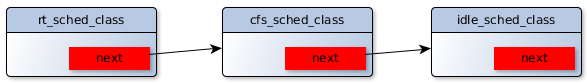
\includegraphics[width=\textwidth]{images/sched_classes}
        \caption{Scheduling classes in Linux}
        \label{fig:sched_classes}
\end{figure}
The basic scheduling unit in Linux is scheduling entity, which can represent
tasks or task groups. There are two kinds of scheduling entities:
\texttt{struct sched\_entity} for cfs scheduling class and 
\texttt{struct sched\_rt\_entity} for rt scheduling class.
When \texttt{CONFIG\_FAIR\_GROUP\_SCHED} is set, cfs task grouping 
is enabled. And \texttt{CONFIG\_RT\_GROUP\_SCHEED} is the kernel configuration
for rt task group scheduling.
\begin{lstlisting}
struct task_struct {
	...
	struct sched_entity se;
	struct sched_rt_entity rt;
	...
};

struct task_group {
#ifdef CONFIG_FAIR_GROUP_SCHED
	/* sched_entity of this group on each cpu */
	struct sched_entity **se;
	...
#endif
#ifdef CONFIG_RT_GROUP_SCHED
	/* sched_rt_entity of this group on each cpu */
	struct sched_entity **rt_se;
	...
#endif
	...
};
\end{lstlisting}

\subsection{Runqueue centered scheduling\label{LinuxSched_rq}}
Every hook in \texttt{struct sched\_class} deals with the data structure 
\texttt{struct rq}, which is called run queue in Linux.  We can say that 
Linux scheduling is runqueue centered. In Linux, the \texttt{struct rq} is 
a per CPU data structure; each cpu is associated with a runqueue. Although 
the name indicates, \texttt{struct rq} is not a queue. Let's have a look at 
the inside of a runqueue structure:
\begin{lstlisting}
struct rq {
	...
	unsigned long nr_running;
	struct cfs_rq cfs;
	struct rt_rq rt;
	struct task_struct *curr, *idle;
	u64 clock;
#ifdef CONFIG_SMP
	int cpu;
#endif
	...
};
\end{lstlisting}
\begin{itemize}
\item \texttt{nr\_running} specifies the number of runnable tasks in the
	runqueue.
\item \texttt{cfs and rt} are two specific runqueues for 
	\texttt{cfs\_sched\_class} and \texttt{rt\_sched\_class} respectively. 
	In order to handle specific type of tasks, different schedulers define 
	new type of runqueue data structures. For example, \texttt{struct cfs 
	rq} and \texttt{struct rt\_rq}. 
\item \texttt{curr} points to the task currently running.
\item \texttt{idle} points to a special idle task when no other tasks are
	runnable.
\item \texttt{clock} is updated by \texttt{update\_rq\_clock} method.
\item \texttt{cpu} tells the CPU of this runqueue.
\end{itemize}

\subsection{Completely Fair scheduler\label{sec:LinuxSched_cfs}}
Completely fair scheduler is implemented in \texttt{fair\_sched\_class}. 
Most tasks inside Linux are scheduled by completely fair scheduling class
 and are normal tasks, which can be further divided into three sub 
types given scheduling policies (\texttt{SCHED\_NORMAL}, \texttt{SCHED\_BATCH}
and \texttt{SCHED\_IDLE\footnote{This SCHED\_IDLE policy is not related to
idle\_sched\_class which aims to handle a special idle task.}}).

CFS tries to distribute CPU cycles fairly to tasks and task groups according
to their \emph{weight}. A specific runqueue structure \texttt{struct cfs\_rq}
is provided to deal with normal tasks. Recall an instance of such cfs runqueue
is embedded in the per CPU runqueue and each task group holds a pointer
to cfs runqueue on each CPU to store tasks belonging to it.
The scheduling entity handled by cfs scheduling class is 
\texttt{struct sched\_entity}. Here instead of studying the details of
CFS, we are going to see how different scheduling components
(\texttt{sched\_entity}, \texttt{task\_struct}, \texttt{task\_group}
and \texttt{struct cfs\_rq}) are related.
\begin{lstlisting}
struct cfs_rq {
        unsigned long nr_running;
        u64 min_vruntime;
        struct rb_root tasks_timeline;
#ifdef CONFIG_FAIR_GROUP_SCHED
        struct rq *rq;  
	struct task_group *tg;
#endif
	...
};
\end{lstlisting}
\begin{itemize}
\item \texttt{nr\_running} is the number of tasks in this cfs runqueue.
\item \texttt{min\_vruntime} tracks the minimum virtual runtime of all
	tasks associated with this cfs runqueue.
\item \texttt{tasks\_timeline} is the root of the red-black tree where 
	all tasks associated with this cfs runqueue is stored. Tasks are 
	ordered by their virtual run time value.
\item \texttt{rq} is the per CPU runqueue this cfs runqueue is embedded in.
\item \texttt{tg} is the task group that owns this cfs runqueue.
\end{itemize}
\begin{lstlisting}
struct sched_entity {
	...
	struct cfs_rq *cfs_rq;
#ifdef CONFIG_FAIR_GROUP_SCHED
	struct cfs_rq *my_q;
#endif
	...
}; 
\end{lstlisting}
\begin{itemize}
\item \texttt{cfs\_rq} is where this entity is to be queued.
\item \texttt{my\_rq} is the cfs runqueue owned by this entity(group).
	Remember that a schedulign entity can also represent a task group.
\end{itemize}
When cfs task group scheduling is enabled. In this case, the cfs scheduling 
scheme is shown in figure\ref{fig:cfs_scheme_tg}. This is not a complete
scheme: 1) Under a task group there could be sub groups, which behave as 
the task in the figure 2) In the system, there is a top group, which includes
all tasks in the system defaultly; tasks in this group are enqueued in the
cfs runqueue embedded in the per CPU runqueue directly.
\begin{figure}[htbp]
        \centering
        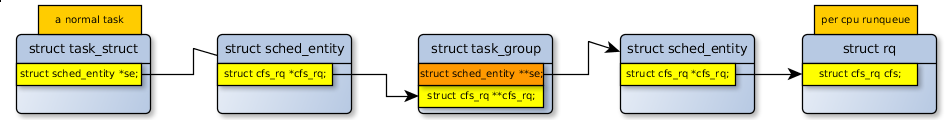
\includegraphics[width=\textwidth]{images/cfs_scheduling_scheme_tg}
        \caption{CFS scheduling when cfs group scheduling is enabled.}
        \label{fig:cfs_scheme_tg}
\end{figure}

If cfs task group scheduling is not enabled, a task is directed to its 
per CPU runqueue by a \emph{task\_rq} marco. \emph{task\_rq} also works 
for rt tasks when rt task group scheduling is not enabled.
\ref{fig:sched_scheme_no_tg}.
\begin{figure}[htbp]
        \centering
        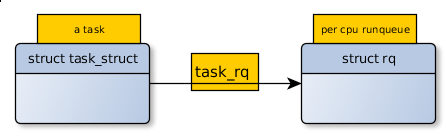
\includegraphics[height=0.1\textheight,width=0.5\textwidth]{images/scheduling_scheme_no_tg}
        \caption{Scheduling scheme without group scheduling}
        \label{fig:sched_scheme_no_tg}
\end{figure}

\subsection{Real time scheduler\label{sec:LinuxSched_rt}}
Tasks with POSIX real time policies \texttt{SCHED\_FIFO} and \texttt{SCHED\_RR}
are scheduled by the real time scheduling class \texttt{rt\_sched\_class} and
are called rt tasks. Given figure\ref{fig:sched_classes}, rt tasks are always
schedueld over normal tasks. 

\texttt{SCHED\_FIFO} implements a simple first-in, first-out scheduling 
algorithm. A running \texttt{SCHED\_FIFO} task can only be preempted by a 
higher priority rt task. \texttt{SCHED\_RR} is \texttt{SCHED\_FIFO} with 
timeslices --- it is a round robin algrithm. When a \texttt{SCHED\_RR}
task exhausts its timeslice, another \texttt{SCHED\_RR} task of the same
priprity is picked to run a timeslice, and so on. In either case, a rt task
cannot be preempted by a lower priority task.

The rt scheduling class provides with a sub runqueue structure 
\texttt{struct rt\_rq} to deal with rt tasks.
\begin{lstlisting}
struct rt_rq {
	struct rt_prio_array active;
        unsigned long rt_nr_running;
#ifdef CONFIG_RT_GROUP_SCHED
        struct rq *rq;
        struct task_group *tg;
#endif
	...
};

struct rt_prio_array {
	DECLARE_BITMAP(bitmap, MAX_RT_PRIO+1); 
	struct list_head queue[MAX_RT_PRIO];
};
\end{lstlisting}
All rt tasks with the same priority are kept in a linked list headed by
$active.queue[prio]$. If there is a task in the liset, the corresponding 
bit in $active.bitmap$ is set.

The connections among \texttt{struct sched\_rt\_entity} and other scheduling
components are similar to the \text{struct sched\_entity} case.
\begin{lstlisting}
struct sched_rt_entity {
	...
	struct rt_rq *rt_rq;
#ifdef CONFIG_RT_GROUP_SCHED
	struct rt_rq *my_q;
#endif
	...
}; 
\end{lstlisting}
When \texttt{CONFIG\_RT\_GROUP\_SCHED} is set, figure\ref{fig:rt_scheme_tg} 
shows the scheduling scheme of rt tasks. If rt task group scheduling is 
not enabled, still \emph{task\_rq} marco will be used.
\begin{figure}[htbp]
        \centering
        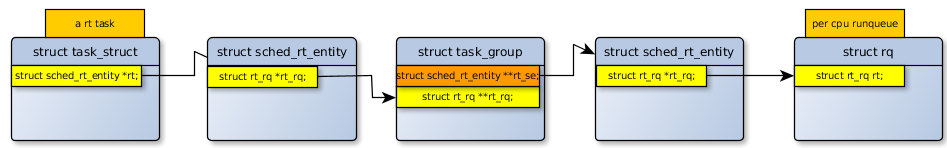
\includegraphics[width=\textwidth]{images/rt_scheduling_scheme_tg}
        \caption{RT scheduling when rt group scheduling is enabled.}
        \label{fig:rt_scheme_tg}
\end{figure}

\section{Related work\label{sec:RelatedWork}}
\subsection{RT throttling\label{sec:RelatedWork_RT}}
Enabling \texttt{CONFIG\_RT\_GROUP\_SCHED} lets users explicitly allocate
CPU bandiwidth to rt tasks in task groups. It uses the \emph{control group}
(cgroup) virtual file system. Each cgroup associates a set of tasks with
a set of resources, called \emph{subsystems}. For example \emph{cpuset} 
subsystem is responsible for assigning a set of CPUs and Memory Nodes to
tasks in a cgroup. Such tasks and resources can be further distributed in 
sub cgroups. Each cgroup is represented by a directory in the cgroup file 
system and a hierarchy of cgroups maps to a hierarchy of directories. In 
the directory, each mounted subsystem provides a list of files that are used 
as interfaces to control the allocation of a resource.
Through mounting the \emph{cpu} subsystem, two interfaces $cpu.rt\_period\_us$ 
and $cpu.rt\_runtime\_us$ are used to control the CPU bandwidth for rt 
tasks in each cgroup. That is, the total execution time of rt tasks in a cgroup 
on each CPU in time length $rt\_period\_us$ cannot exceed $rt\_runtime\_us$. 
If this constraint is met, rt tasks would not be choosen to run on that CPU 
until a new period; we call such tasks be throttled.

No matter \texttt{CONFIG\_RT\_GROUP\_SCHED} is set or not, in order to avoid rt 
tasks forever occupy thc CPU, there is a system wide setting that constraints
rt tasks' execution through the /proc virtual file system :

	$/proc/sys/kernel/sched\_rt\_period\_us$ 

	$/proc/sys/kernel/sched\_rt\_runtime\_us$ 
\\This applies to all rt tasks in a system.

\subsection{CFS bandwidth control\label{RelatedWork_CFS}}
Basically, CFS bandwidth control is the same technique as RT throttling
applying on normal tasks. It is a \texttt{CONFIG\_FAIR\_GROUP\_SCHED} 
extension which allows the specification of the maximum CPU bandwidth
available to normal tasks  in a cgroup or cgroup hierarchy.
The bandwidth allowed to a cgroup is specified using a 
quota(\texttt{cpu.cfs\_quota\_us}) and a period(\texttt{cpu.cfs\_period\_us}).
By specifying this, normal tasks in a cgroup will be limited to 
\texttt{cfs\_quota\_us} units of CPU time within the period of 
\texttt{cfs\_period\_us}. Recall that in RT throttling \ref{sec:RelatedWork_RT},
the reserved bandwidth through cgroup interfaces are applied in each CPU
individually.
\subsection{AQuoSA\label{sec:AQuoSA}}
The Adaptive Quality of Service Architecture composes two parts: 
a resource reservation scheduler an a feedback-based
control mechanism. The scheduler uses CBS rules to rserve CPU bandwidth for
a task, which is a rt task with SCHED\_RR policy in its Linux implementation.
Given the error between the reserved computation and the amount of CPU cycles
really consumed, the feedback controller adapts CBS reservation paramters to
provide quality of service CPU allocation in the system.
The control mechanism depends on CBS performance, not the scheduling details.
That is, such a control mechanism can be applied to general CBS based 
scheduling. AQuoSA lacks considerations on multi-processor platform.
  
\subsection{Schedule-deadline patch}
The schedule-deadline patch for Linux kernel is being developed to extend
current mainline Linux with a deadline-based scheduling method. 
In schedule-deadline, a new scheduling class (scheduler) is implemented and 
has highest priority among all scheduling classes. Tasks scheduled by this
scheduling class are called sched tasks. A sched task is assigned deadlines
according to CBS rules and scheduled in ''earliest deadline first (EDF)'' way.
\subsection{IRMOS real-time framework}
The rague name IRMOS comes from the European project ''Interactive Real-time
Multimedia Applications on Service Oriented Infrastructures''. 
The IRMOS 
framework replace rt throttling mechanism in mainline Linux with real time
CPU reservation(still CBS), and reuses the existing interfaces. So, users 
configure the cgroup interface as what we saw in rt 
throttling(\ref{sec:RelatedWork_RT}), the difference is that this time the CPU 
bandwidth is allocated in a guaranteed way. Also, new cgroup interfaces are 
added to assist reserved CPU power distribution in the cgroup hierarchy.

\subsection{Motivation from previous work\label{sec:motivation}}
Based on Linux, CPU bandwidth control can be applied in the level of 
single tasks or task groups which are shceudled by some policies.
Such control can be real-time or non real-time. 
One obervation here is that there does not exist a mechanism that can 
control CPU bandwidth for all kinds of tasks as a whole. 
Such a general control mechanism is the initial consideration of 
OXC framework. 
